% Section 2.3: The Fermi Large Area Telescope
% Structure: Introduction -> Instrument Overview -> IRFs -> Data Products and Catalogs

\section{The Fermi Large Area Telescope}
\label{sec:fermi_lat_section}
The overlapping source populations, diffuse foregrounds, and the faint unresolved emission described in the previous section place specific demands on both the detecting instrument and the data analysis pipeline.
To interpret the astrophysical gamma-ray sky, we must first understand the telescope that observes it.
Launched in 2008, the \textit{Fermi} Large Area Telescope (LAT) has provided the most sensitive all-sky survey in the GeV domain to date, operating continuously for over fifteen years.
While the detailed pipelines for data extraction and analysis are discussed directly within the subsequent chapters, it is necessary to establish the basic instrumental parameters and data products that define the practical limits of current observations.
In this section, we review the fundamental design of the LAT, the energy-dependent instrumental response functions that govern its spatial and energy resolution, and the resulting catalogs of point sources that serve as the foundation for both individual target searches and statistical population studies.

\subsection{Instrument Overview}
\label{sec:fermi_lat}

The \textit{Fermi} Large Area Telescope (LAT) is a pair-conversion telescope designed to measure cosmic gamma rays.
Because high-energy gamma rays cannot be reflected or refracted, they must be detected indirectly through their interaction with matter.
Fermi-LAT is therefore structured around four primary subsystems that convert incident photons into charged particles, track their trajectories, measure their energy, and reject the overwhelming background of cosmic rays \cite{Atwood:2009ez}.
Figure~\ref{fig:lat_schematic} illustrates the instrument components.

\begin{figure}[t]
	\centering
	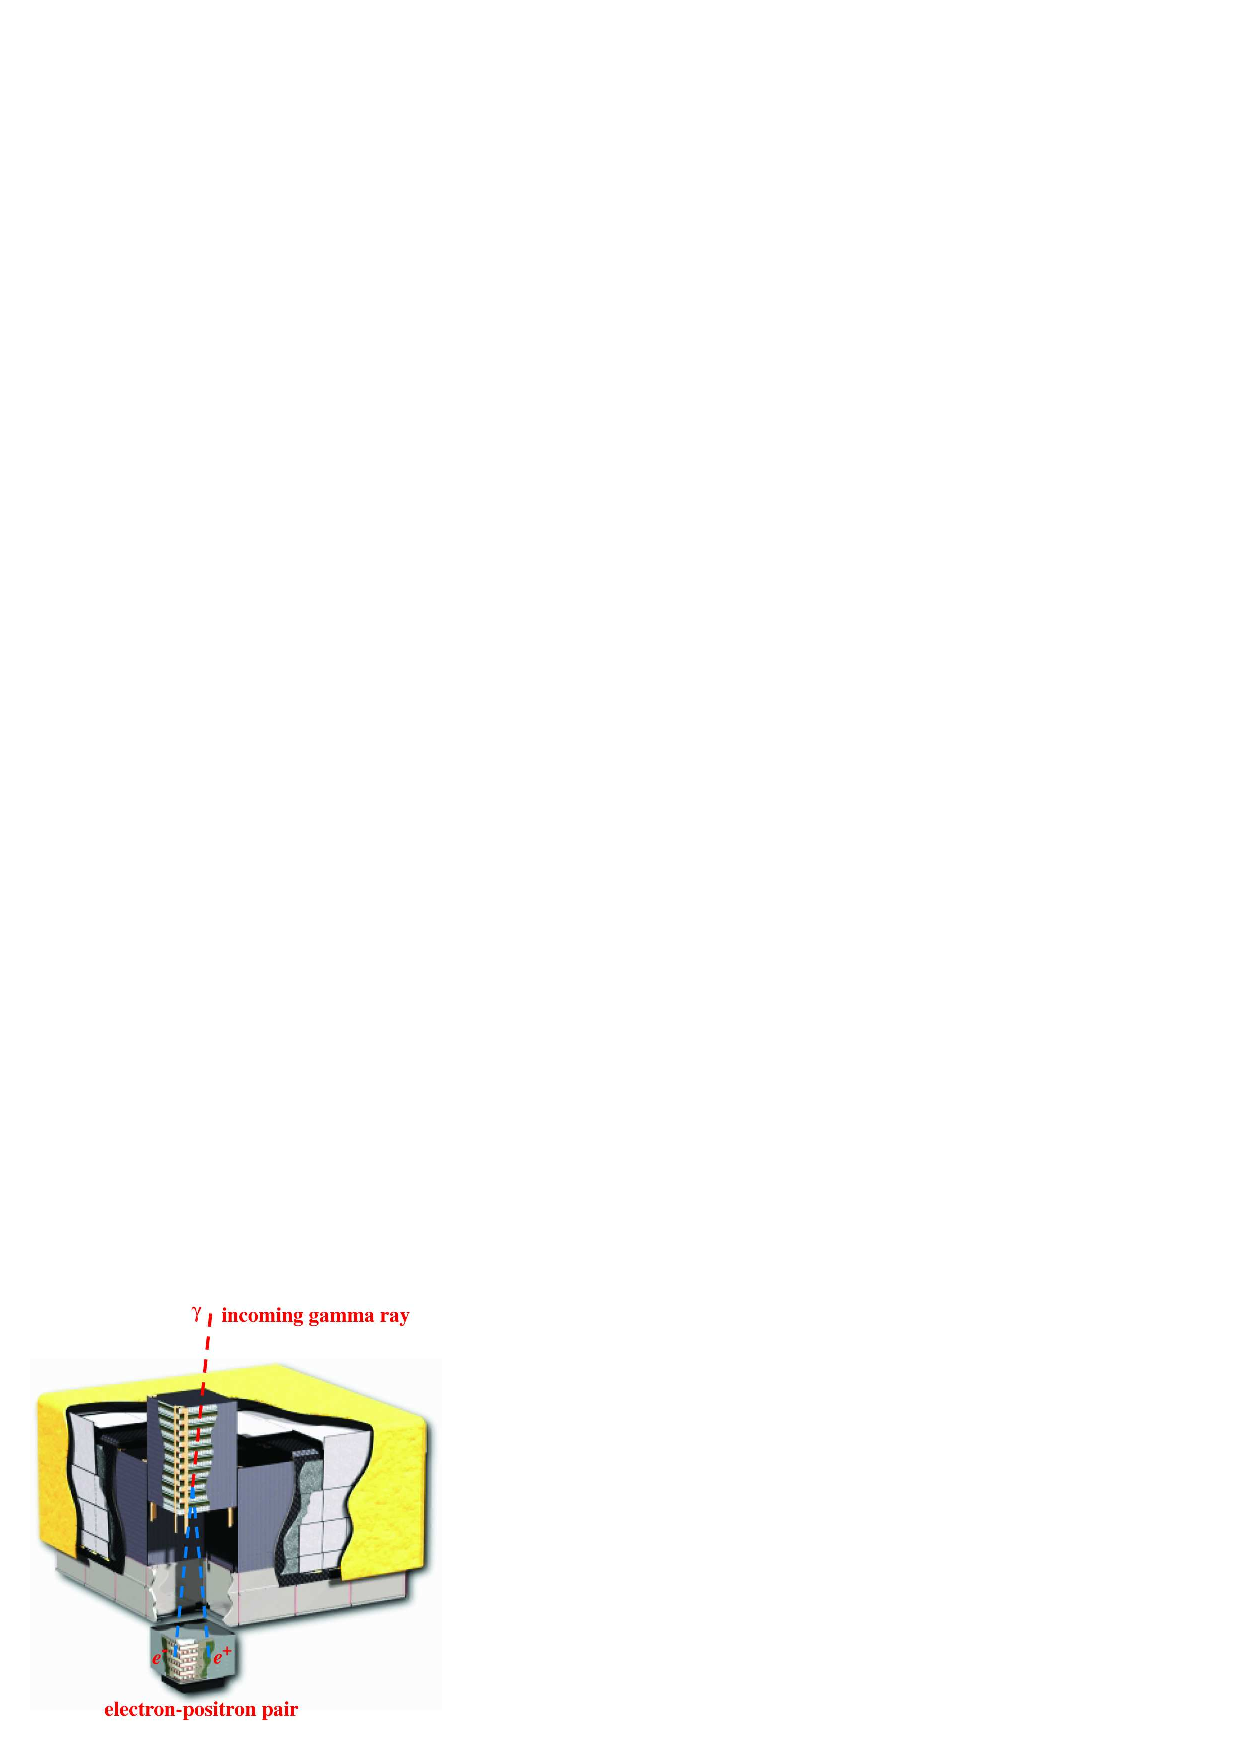
\includegraphics[width=0.5\columnwidth]{chapter_02/figures/lat_schematic.pdf}
	\caption{Schematic diagram of the Large Area Telescope, showing the tracker modules, calorimeter, and the surrounding Anticoincidence Detector.
		The telescope's dimensions are $1.8~\mathrm{m} \times 1.8~\mathrm{m} \times 0.72~\mathrm{m}$.
		Adapted from Figure 1 from \cite{Atwood:2009ez}.
	}
	\label{fig:lat_schematic}
\end{figure}

The conversion process takes place in the precision tracker, which consists of a $4 \times 4$ array of 16 modules.
Each module contains 18 $x,y$ tracking planes of single-sided silicon microstrip detectors, interleaved with high-$Z$ tungsten conversion foils.
An incoming gamma ray preferentially undergoes pair production within the tungsten, yielding an electron-positron ($e^+e^-$) pair.
The silicon strip detectors then record the passage of these charged particles through successive layers.
By precisely tracing the particle tracks back to their common vertex, the instrument reconstructs the arrival direction of the original photon.

Below the tracker lies the calorimeter, composed of 96 cesium iodide (CsI(Tl)) scintillating crystals per module, arranged in a configuration of 8 layers with alternating orientation.
% The total calorimeter depth is 8.6 radiation lengths, bringing the full instrument depth to 10.1 radiation lengths.
The calorimeter measures the total energy deposited by the electromagnetic shower and images its longitudinal and transverse development profile.
This three-dimensional shower imaging is essential not only for energy reconstruction---allowing measurements to extend beyond the calorimeter's physical depth up to TeV energies---but also for background rejection, as it separates the narrow electromagnetic showers from photon-induced events from the broader hadronic cascades produced by cosmic rays.

The entire tracker array is covered by the Anticoincidence Detector (ACD), a segmented shield of 89 plastic scintillator tiles read out by wavelength-shifting fibers and photomultiplier tubes.
The ACD provides a charged-particle detection efficiency exceeding 0.9997 averaged over its area, enabling rejection of the charged cosmic-ray background that outnumber gamma rays by several orders of magnitude \cite{Atwood:2009ez}.
The segmentation of the ACD is necessary to suppress the ``backsplash'' effect: at high energies, secondary particles from electromagnetic showers in the calorimeter can scatter back into the shield, creating false veto signals.
By considering only the ACD segment nearest the candidate photon's entry point, the instrument avoids falsely rejecting valid high-energy gamma-ray events.

This hardware configuration enables the LAT to achieve substantial improvements over previous-generation instruments.
The LAT operates across an energy range spanning from 20~MeV to over 300~GeV.
Its compact aspect ratio grants a large field of view of approximately 2.4~sr at 1~GeV, ensuring that nearly all pair-conversion events initiated in the tracker pass into the calorimeter for energy measurement.
In its primary survey mode, the spacecraft rocks alternately by $\pm 35^\circ$ from the zenith on consecutive orbits, achieving nearly uniform exposure of the entire sky every two orbits---approximately three hours.
Combined with a peak effective area of $\sim$9,500~cm$^2$ at normal incidence and a dead time of only 26.5~$\mu$s per event readout, these capabilities result in a sensitivity approximately 25 times greater than EGRET, enabling the detection and characterization of thousands of faint source populations \cite{Atwood:2009ez}.

\subsection{Instrument Response Functions}
\label{sec:irfs}

The physical characteristics of the LAT---its tracking efficiency, multiple scattering within the conversion foils, and incomplete shower containment---are encapsulated in the Instrument Response Functions (IRFs).
The IRFs map the true energy, direction, and conversion location of incident gamma rays to their reconstructed quantities.
Three IRF components are particularly relevant for the analyses in this thesis: the Point Spread Function, the energy dispersion, and the effective area.

The Point Spread Function (PSF) describes the angular resolution of the telescope, quantifying the probability distribution of reconstructed directions around the true source position.
At energies below a few GeV, the resolution is dominated by the multiple Coulomb scattering of the newly produced electron-positron pair as it traverses the tungsten conversion foils.
Consequently, the PSF is strongly energy-dependent, as shown in Figure~\ref{fig:lat_psf}: at 100~MeV, the 68\% containment radius spans approximately $3.5^\circ$ to $5^\circ$; it tightens to roughly $0.6^\circ$ at 1~GeV and reaches an asymptotic limit of less than $0.15^\circ$ above 10~GeV \cite{Atwood:2009ez}.
Off-axis, the containment radius degrades by up to a factor of 1.7 at $55^\circ$ incidence.
The broad PSF at lower energies creates a severe source confusion limit: because the spatial profiles of nearby point sources overlap with each other and with the intense Galactic diffuse emission, it becomes statistically difficult to disentangle individual faint objects.
This confusion directly limits the depth of point-source catalogs and motivates the use of statistical population methods---such as those developed in Chapters~\ref{ch:6} and~\ref{ch:7}---rather than standard source-by-source extraction.

\begin{figure}[t]
	\centering
	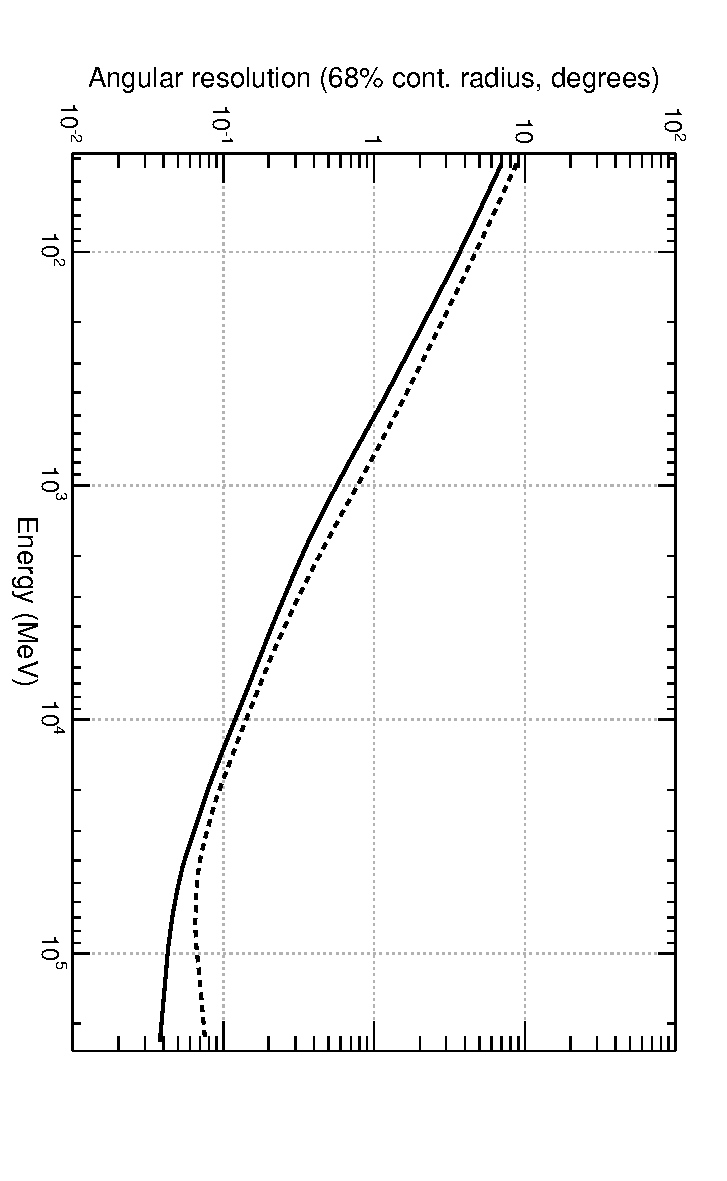
\includegraphics[width=0.5\columnwidth, angle=90]{chapter_02/figures/lat_psf.pdf}
	\caption{The 68\% containment radius of the Point Spread Function as a function of energy at normal incidence (solid) and at $60^\circ$ off-axis (dashed), for photons converting in the thin \textit{front} section of the tracker.
	Photons converting in the thick \textit{back} section have a PSF approximately twice as wide at 1~GeV.
	Credit: Figure 17 from \cite{Atwood:2009ez}.
	}
	\label{fig:lat_psf}
\end{figure}

The energy dispersion quantifies the accuracy of the reconstructed photon energy.
It is determined by the calorimeter's ability to contain and measure the electromagnetic shower.
For on-axis photons, the equivalent Gaussian $1\sigma$ energy resolution ranges from 9\% to 15\% in the 100~MeV--1~GeV band, improves to 8\%--9\% between 1 and 10~GeV, and then degrades to $\sim$18\% near 300~GeV as shower leakage from the finite calorimeter depth becomes significant \cite{Atwood:2009ez}.
At large off-axis angles ($>60^\circ$), where the effective calorimeter depth increases, the resolution can improve to $\sim$6\% above 10~GeV.
For most analyses in this thesis, the energy resolution is sufficiently precise that energy dispersion is not a dominant systematic.

Not every gamma ray that enters the LAT produces a usable event: some pass through without converting, others are rejected during background filtering.
The effective area captures this by expressing the instrument's photon-collecting power as the area of an ideal, perfectly efficient detector that would record the same number of events.
At normal incidence, it rises steeply from $\sim$100~cm$^2$ at 20~MeV to a broad plateau of $\sim$8,000--9,500~cm$^2$ between 1~GeV and several hundred GeV, before declining at the highest energies \cite{Atwood:2009ez}.
For comparison, the LAT's overall footprint is $1.8 \times 1.8~\mathrm{m}^2$; the peak effective area of $\sim$9,500~cm$^2$---roughly a third of the geometric area---reflects the compounded probabilities of pair conversion in the tungsten, successful track reconstruction, and survival of background-rejection cuts.
For a survey instrument like the LAT, however, what matters is not just how efficiently it detects photons from a single direction, but how much sky it can monitor simultaneously.
The \emph{acceptance}---the effective area integrated over the instrument's field of view---captures both factors at once.
The LAT's acceptance peaks at $\sim$2.5~m$^2$~sr above 1~GeV, meaning the telescope collects photons as if it were a perfect $2.5~\mathrm{m}^2$ detector watching one steradian of sky, or equivalently a smaller detector watching a proportionally wider region.
To put this in perspective, the third EGRET catalog contained only 271 sources; the LAT's much larger acceptance, combined with its suppression of the backsplash self-veto that crippled EGRET above 10~GeV, is the primary reason the LAT has been able to catalog thousands \cite{Atwood:2009ez}.

The accuracy of the IRFs relies directly on the underlying event reconstruction algorithms.
The Pass~8 analysis framework represents a comprehensive overhaul of the LAT event-level reconstruction, designed to maximize the scientific return of the data \cite{Fermi-LAT:2013jgq}.
A major improvement in Pass~8 was the mitigation of ``ghost signals''---instrumental pile-up and out-of-time residual hits from previous events that previously degraded the reconstruction.
% By introducing tree-based tracking in the tracker and Minimum Spanning Tree clustering in the calorimeter, Pass~8 successfully separated these artifacts from genuine gamma-ray showers.
This enabled a significant expansion of the effective area, particularly below 100~MeV and above 1~TeV, while simultaneously reducing background contamination.
Pass~8 also introduced event subclassifications that partition data by the quality of the reconstructed direction (PSF event types: PSF0--PSF3, from broadest to narrowest) and the quality of the energy measurement (EDISP event types).
This partitioning allows analyses to select event classes optimized for their specific scientific goals---angular resolution for morphological studies, or photon statistics for spectral analyses.

Subsequent iterations, most notably the P8R3 release \cite{Bruel:2018lac}, further refined the residual background rejection, producing a spatially uniform and clean dataset that serves as the baseline for all modern \textit{Fermi}-LAT analyses, including the work presented in this thesis.

\subsection{Data Products and Catalogs}
\label{sec:data_products}
With the IRFs established, we now turn to how the LAT data are translated into astrophysical catalogs.
Converting raw photon events into measurements of individual sources requires disentangling point-like objects from the structured diffuse backgrounds.
The \textit{Fermi}-LAT collaboration achieves this through a maximum likelihood framework \cite{Mattox:1996zz,Fermi-LAT:2019yla}.
The observed sky is modeled as a linear combination of spatial and spectral templates: the highly structured Galactic diffuse emission, a spatially uniform isotropic component capturing the extragalactic background and residual instrumental noise, and individual point sources each parametrized by a position and spectral model.
The normalizations and spectral parameters of all components are simultaneously adjusted to maximize the Poisson likelihood function against the observed photon counts across the sky.

To evaluate the significance of a candidate point source, the framework computes the Test Statistic (TS), defined as \[ TS = 2\ln\frac{\mathcal{L}_1}{\mathcal{L}_0}, \] where $\mathcal{L}_1$ is the maximum likelihood of the model with the candidate source included and $\mathcal{L}_0$ is the maximum likelihood of the null hypothesis without it \cite{Mattox:1996zz}.
By Wilks' theorem, $TS$ is approximately distributed as $\chi^2$ with a number of degrees of freedom equal to the additional free parameters of the source model.
For a point source with four free parameters (two spatial and two spectral), the catalog detection threshold of $TS > 25$ corresponds to a significance of just over $4\sigma$ \cite{Fermi-LAT:2015bhf,Fermi-LAT:2019yla}.
As a practical rule of thumb, for an isolated source with known position (one spectral degree of freedom), the significance is well approximated by $\sqrt{TS}\,\sigma$.
This threshold defines the boundary between what is considered a ``resolved'' source entering the catalog and what remains part of the unresolved diffuse background.

The results of these analyses have been systematically compiled into a series of catalogs of increasing depth.
The progression from the First \textit{Fermi}-LAT Catalog (1FGL, based on 11 months of data) through the Third Catalog (3FGL, 4 years, 3,033 sources) to the Fourth Catalog (4FGL, 8 years, 5,064 sources) \cite{Fermi-LAT:2015bhf,Fermi-LAT:2019yla} reflects both the accumulation of exposure and successive improvements in event reconstruction and background modeling.
The most recent published incremental release, 4FGL-DR4, extends the dataset to 14 years and contains 7,194 sources \cite{2023arXiv230712546B}, with more recent data releases continuing to grow the catalog.
Throughout this evolution, the detection threshold has remained at $TS > 25$, so the growing source count is driven primarily by longer exposure and improved sensitivity from Pass~8 event reconstruction.

Each catalog entry reports the source localization (with 95\% confidence ellipse), the integrated energy flux in multiple bands, the best-fit spectral model, a variability index, and multi-wavelength associations.
The spectral models employed include the simple power law, the log-parabola (commonly preferred for blazars), and the power law with an exponential cutoff (standard for pulsars).
These spectral characterizations, together with variability and localization accuracy, form the feature space used in Chapter~\ref{ch:5} for the machine-learning classification of unassociated sources.

The association procedure matches each gamma-ray source against catalogs at radio, infrared, optical, and X-ray wavelengths using Bayesian and likelihood-ratio methods.
Sources receiving a high-confidence match are labeled as ``associated''; those with firm identification through periodicity, correlated variability, or resolved angular extent are labeled as ``identified.'' In the 4FGL, more than 3,130 sources are identified or associated with active galaxies of the blazar class, while pulsars represent the largest Galactic source class.
However, a substantial fraction---1,336 sources (26\%) in the base 4FGL---lacks any plausible multi-wavelength counterpart and remains unassociated \cite{Fermi-LAT:2019yla}.
These unassociated sources are concentrated along the Galactic plane, where the dense background complicates counterpart searches, and at high latitudes, where their average spectral properties resemble those of blazars of unknown type.

This large population of unassociated sources is scientifically important for multiple reasons.
Beyond its likely composition of faint blazars and pulsars below the sensitivity of current multi-wavelength surveys, it also constitutes the primary search pool for exotic gamma-ray emitters such as dark matter subhalos.
As discussed in Chapter~1, $\Lambda$CDM cosmology predicts the existence of thousands of Galactic subhalos below $\sim 10^7\,M_\odot$---too low in mass to retain gas or form stars, and therefore invisible at all wavelengths except gamma rays, where WIMP annihilation could produce a faint, spectrally soft signal closely resembling an unassociated \textit{Fermi}-LAT point source \cite{Cirelli:2024ssz, Springel:2008cc}. Separating such candidates from the astrophysical contaminants within the 4FGL catalog is the central challenge addressed in Chapter~\ref{ch:5}, where machine learning techniques are used to search for dark matter subhalo candidates among the unassociated sources.
